\clearpage

\renewcommand{\thefigure}{A\arabic{figure}}
\setcounter{figure}{0}
\renewcommand{\thetable}{A.\arabic{table}}
\setcounter{table}{0}
\renewcommand{\thesection}{A.\arabic{section}}
\setcounter{section}{0}

\section*{\textbf{Appendix}}

\subsection*{Additional Replication Information}

\subsubsection*{Gibler (2017)}

%
% latex table generated in R 3.4.1 by xtable 1.8-2 package
% Sat Oct 21 23:10:24 2017
\begin{table}[ht]
\centering
\begingroup\normalsize
\begin{tabular}{lccc}
 Variable & GLM (Logit) & GLM (Probit) & AME \\ 
  \hline
\hline
(Intercept) & $-5.826$ & $-2.793$ & $-2.758$ \\
   & (0.366) & (0.366) & (0.045) \\ 
  Allied & 0.133 & 0.067 & $0.078$ \\
   & (0.102) & (0.102) & (0.021) \\ 
  Joint Democracy & $-0.527$ & $-0.186$ & 0.005 \\
   & (0.099) & (0.099) & (0.022) \\ 
  Peace Years & $-0.261$ & $-0.099$ & $-0.058$ \\
   & (0.016) & (0.016) & (0.004) \\ 
  Spline 1 & $-0.001$ & $0.000$ & $0.000$ \\
   & (0.000) & (0.000) & (0.000) \\ 
  Spline 2 & $0.000$ & $0.000$ & $0.000$ \\
   & (0.000) & (0.000) & (0.000) \\ 
  Spline 3 & 0.000 & 0.000 & $0.000$ \\
   & (0.000) & (0.000) & (0.000) \\ 
  Contiguity & $2.427$ & $0.95$ & $0.66$ \\
   & (0.196) & (0.196) & (0.023) \\ 
  Parity & -0.77 & -0.228 & -0.067 \\ 
   & (0.551) & (0.551) & (0.057) \\ 
  Parity at Entry Year & $2.034$ & 0.739 & -0.05 \\
   & (0.617) & (0.617) & (0.065) \\ 
  Rivalry & $2.034$ & $1.035$ & $0.655$ \\
   & (0.213) & (0.213) & (0.028) \\ 
   \hline
\hline
\end{tabular}
\endgroup
\caption{Parameter comparison for Gibler (2017). Standard errors in parentheses.} 
\label{tab:gibler_coef}
\end{table}

\FloatBarrier

\begin{figure}
	\centering   
	\subfigure[AUC]{\label{fig:giblerroc}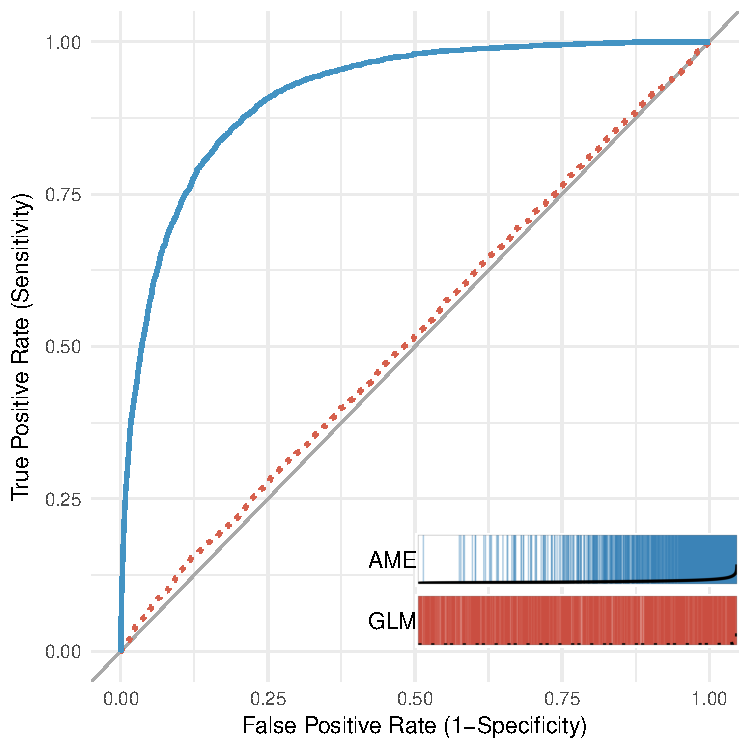
\includegraphics[width=.45\textwidth]{gibler_roc_outSample.pdf}}
	\subfigure[Precision and Recall]{\label{fig:giblerpr}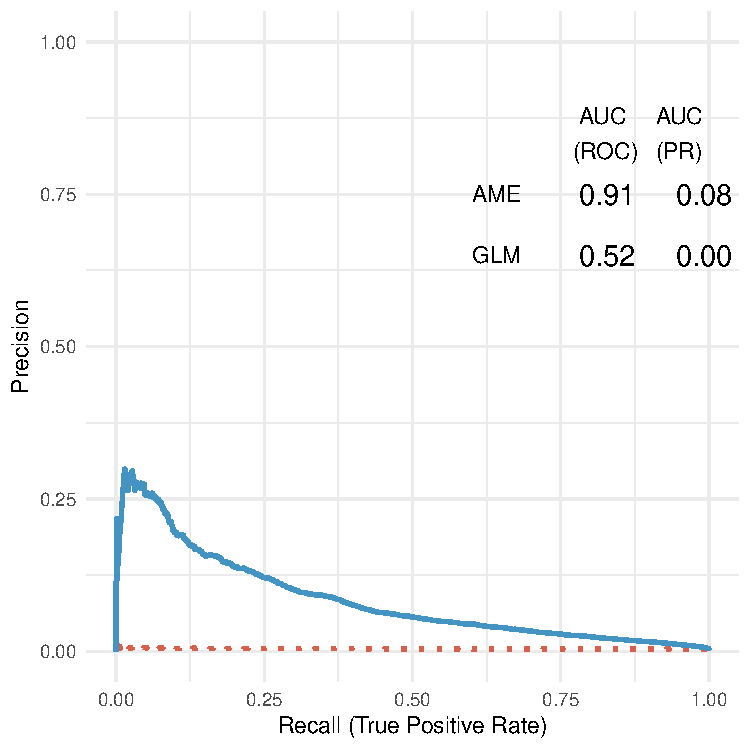
\includegraphics[width=.45\textwidth]{gibler_pr_outSample.pdf}}
	\caption{Assessments of out-of-sample predictive performance for Gibler (2017) using ROC curves and PR curves.}
\end{figure}
\FloatBarrier

\clearpage
\subsubsection*{McDonald (2004)}

%Coefficient plot and performance comparison.

% latex table generated in R 3.4.1 by xtable 1.8-2 package
% Sat Oct 21 23:10:32 2017
\begin{table}[ht]
\centering
\begingroup\normalsize
\begin{tabular}{lccc}
 Variable & GLM (Logit) & GLM (Probit) & AME \\ 
  \hline
\hline
(Intercept) & 0.054 & 0.085 & $-1.171^{\ast\ast}$ \\ 
   & (1.179) & (0.409) & (0.096) \\ 
  Spline0 & $-0.438^{\ast\ast}$ & $-0.222^{\ast\ast}$ & $-0.145^{\ast\ast}$ \\ 
   & (0.061) & (0.026) & (0.019) \\ 
  Spline1 & $-0.003^{\ast\ast}$ & $-0.002^{\ast\ast}$ & $-0.001^{\ast\ast}$ \\ 
   & (0.001) & (0.000) & (0.000) \\ 
  Spline2 & 0.001 & $0.001^{\ast\ast}$ & $0.000^{\ast}$ \\ 
   & (0.001) & (0.000) & (0.000) \\ 
  Spline3 & 0.000 & 0.000 & $0.000^{\ast\ast}$ \\ 
   & (0.000) & (0.000) & (0.000) \\ 
  Shared Alliance & $0.483^{\ast\ast}$ & 0.155 & $0.342^{\ast\ast}$ \\ 
   & (0.233) & (0.095) & (0.069) \\ 
  Contiguous & $2.011^{\ast\ast}$ & $0.789^{\ast\ast}$ & $0.988^{\ast\ast}$ \\ 
   & (0.343) & (0.118) & (0.066) \\ 
  Log Capabilities Ratio & $-0.146^{\ast\ast}$ & $-0.054^{\ast\ast}$ & $0.029^{\ast\ast}$ \\ 
   & (0.072) & (0.026) & (0.013) \\ 
  Trade Dependence & -22.244 & -7.051 & $-13.134^{\ast\ast}$ \\ 
   & (15.184) & (5.536) & (4.938) \\ 
  Preconflict GDP Change & $-6.79^{\ast\ast}$ & $-3.155^{\ast\ast}$ & $-2.651^{\ast\ast}$ \\ 
   & (2.033) & (0.788) & (0.574) \\ 
  Lowest Dyadic Polity Score & $-0.036^{\ast\ast}$ & $-0.014^{\ast\ast}$ & $-0.026^{\ast\ast}$ \\ 
   & (0.015) & (0.006) & (0.002) \\ 
  Capabilities & $-0.995^{\ast\ast}$ & $-0.349^{\ast\ast}$ & 0.022 \\ 
   & (0.377) & (0.14) & (0.079) \\ 
  Logged GDP & $0.000^{\ast\ast}$ & $0.000^{\ast\ast}$ & $0.000^{\ast\ast}$ \\ 
   & (0.000) & (0.000) & (0.000) \\ 
  Logged Cap. Distance & $-0.425^{\ast\ast}$ & $-0.224^{\ast\ast}$ & $-0.275^{\ast\ast}$ \\ 
   & (0.14) & (0.047) & (0.012) \\ 
  Major Power In Dyad & $0.769^{\ast\ast}$ & $0.312^{\ast\ast}$ & $0.212^{\ast\ast}$ \\ 
   & (0.322) & (0.122) & (0.098) \\ 
  Higest Barrier To Trade & $0.024^{\ast\ast}$ & $0.011^{\ast\ast}$ & $0.004^{\ast\ast}$ \\ 
   & (0.008) & (0.003) & (0.001) \\ 
   \hline
\hline
\end{tabular}
\endgroup
\caption{Parameter comparison for McDonald (2004). Standard errors in parentheses. $^{**}$ and $^{*}$ indicate significance at $p<0.05$ and $p<0.10$, respectively.} 
\label{tab:mcdonald_coef}
\end{table}

\FloatBarrier

\begin{figure}
	\centering   
	\subfigure[AUC]{\label{fig:mcdonaldroc}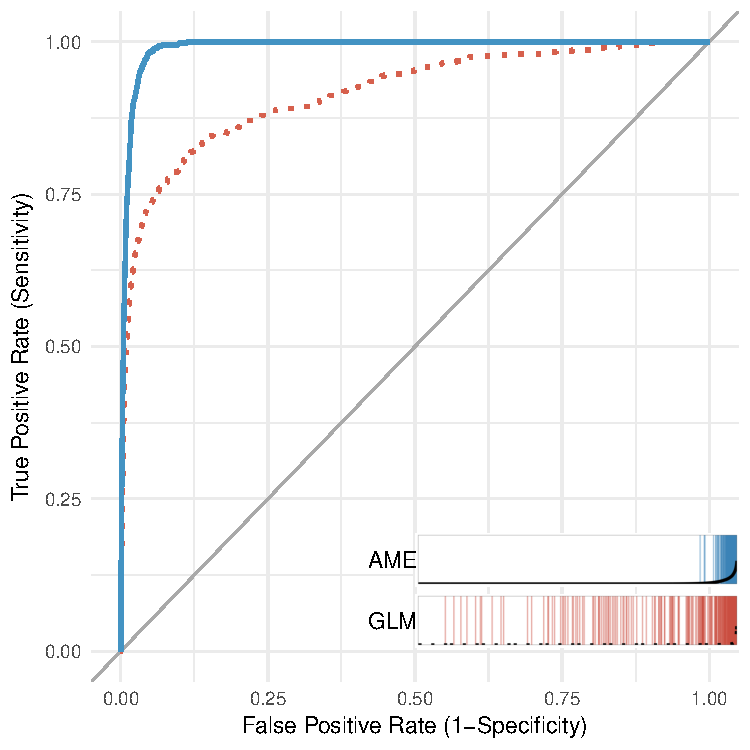
\includegraphics[width=.45\textwidth]{mcdonald_roc_outSample.pdf}}
	\subfigure[Precision and Recall]{\label{fig:mcdonaldpr}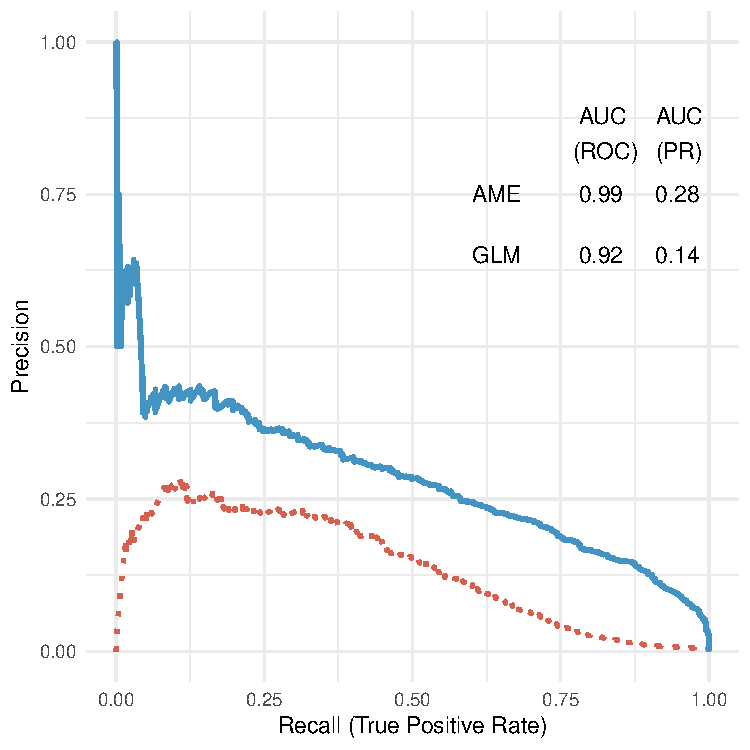
\includegraphics[width=.45\textwidth]{mcdonald_pr_outSample.pdf}}
	\caption{Assessments of out-of-sample predictive performance for McDonald (2004) using ROC curves and PR curves.}
\end{figure}
\FloatBarrier

\clearpage
\subsubsection*{Reiter \& Stam (2003)}

%Coefficient plot and performance comparison.

% latex table generated in R 3.4.1 by xtable 1.8-2 package
% Sat Oct 21 23:16:42 2017
\begin{table}[ht]
\centering
\begingroup\normalsize
\begin{tabular}{lccc}
 Variable & GLM (Logit) & GLM (Probit) & AME \\ 
  \hline
\hline
Intercept & $-4.784^{\ast\ast}$ & $-2.339^{\ast\ast}$ & $-3.144^{\ast\ast}$ \\ 
   & (0.097) & (0.034) & (0.06) \\ 
  Pers/Democ Directed Dyad & $1.026^{\ast\ast}$ & $0.378^{\ast\ast}$ & $0.255^{\ast\ast}$ \\ 
   & (0.14) & (0.051) & (0.068) \\ 
  Democ/Pers Directed Dyad & 0.083 & 0.033 & 0.112 \\ 
   & (0.191) & (0.066) & (0.079) \\ 
  Personal & 0.281 & 0.15 & $0.211^{\ast}$ \\ 
   & (0.265) & (0.099) & (0.11) \\ 
  Military & -0.323 & -0.105 & -0.025 \\ 
   & (0.574) & (0.204) & (0.249) \\ 
  Single & $-0.677^{\ast\ast}$ & $-0.261^{\ast\ast}$ & -0.07 \\ 
   & (0.144) & (0.062) & (0.073) \\ 
  Democracy & $-1.073^{\ast\ast}$ & $-0.428^{\ast\ast}$ & $-0.254^{\ast\ast}$ \\ 
   & (0.194) & (0.07) & (0.063) \\ 
  Contiguous & $2.912^{\ast\ast}$ & $1.147^{\ast\ast}$ & $1.296^{\ast\ast}$ \\ 
   & (0.09) & (0.031) & (0.033) \\ 
  Major Power & $2.174^{\ast\ast}$ & $0.919^{\ast\ast}$ & $0.906^{\ast\ast}$ \\ 
   & (0.101) & (0.037) & (0.093) \\ 
  Ally & 0.078 & -0.003 & $0.136^{\ast\ast}$ \\ 
   & (0.086) & (0.035) & (0.037) \\ 
  Higher/Lower Power Ratio & $-0.316^{\ast\ast}$ & $-0.122^{\ast\ast}$ & $-0.111^{\ast\ast}$ \\ 
   & (0.027) & (0.01) & (0.011) \\ 
  Economically Advanced & -0.175 & -0.054 & 0.053 \\ 
   & (0.131) & (0.051) & (0.05) \\ 
  Years Since Last Dispute & $-0.381^{\ast\ast}$ & $-0.149^{\ast\ast}$ & $-0.129^{\ast\ast}$ \\ 
   & (0.023) & (0.009) & (0.008) \\ 
  Cubic Spline 1 & $-0.004^{\ast\ast}$ & $-0.001^{\ast\ast}$ & $-0.001^{\ast\ast}$ \\ 
   & (0.000) & (0.000) & (0.000) \\ 
  Cubic Spline 2 & $0.002^{\ast\ast}$ & $0.001^{\ast\ast}$ & $0.001^{\ast\ast}$ \\ 
   & (0.000) & (0.000) & (0.000) \\ 
  Cubic Spline 3 & $-0.001^{\ast\ast}$ & $0.000^{\ast\ast}$ & $0.000^{\ast\ast}$ \\ 
   & (0.000) & (0.000) & (0.000) \\ 
   \hline
\hline
\end{tabular}
\endgroup
\caption{Parameter comparison for Reiter \& Stam (2003). Standard errors in parentheses. $^{**}$ and $^{*}$ indicate significance at $p<0.05$ and $p<0.10$, respectively.} 
\label{tab:reiter_stam_coef}
\end{table}
\FloatBarrier

\begin{figure}
	\centering   
	\subfigure[AUC]{\label{fig:reiterstamroc}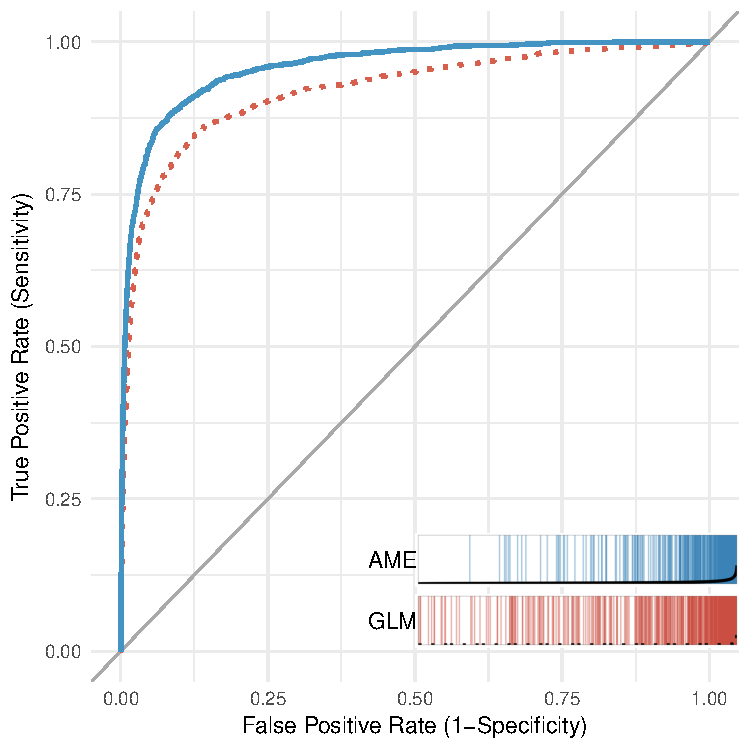
\includegraphics[width=.45\textwidth]{reiter_stam_roc_outSample.pdf}}
	\subfigure[Precision and Recall]{\label{fig:reiterstampr}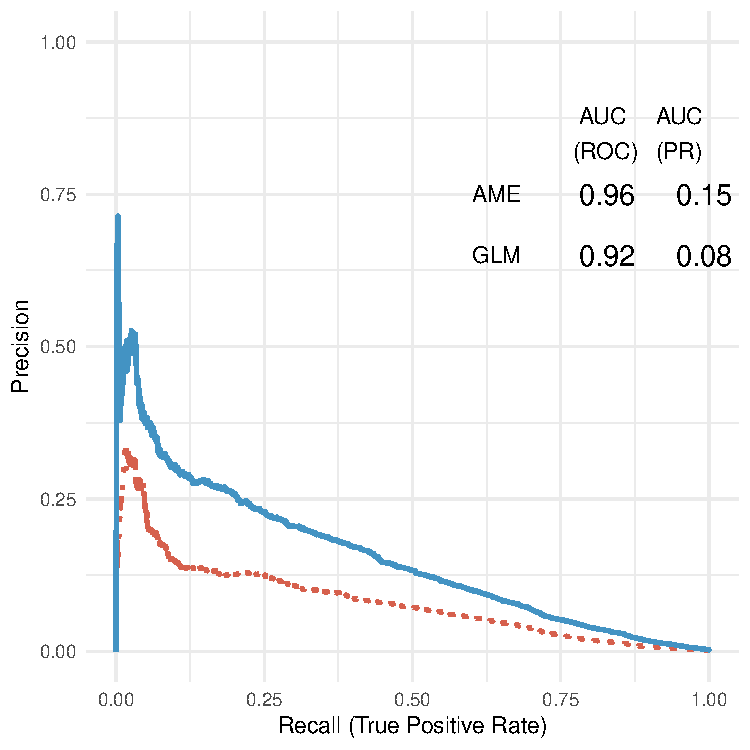
\includegraphics[width=.45\textwidth]{reiter_stam_pr_outSample.pdf}}
	\caption{Assessments of out-of-sample predictive performance for Reiter \& Stam (2003) using ROC curves and PR curves.}
\end{figure}
\FloatBarrier

\clearpage
\subsubsection*{Rose (2004)}

%Coefficient plot and performance comparison.

% latex table generated in R 3.4.1 by xtable 1.8-2 package
% Sat Oct 21 22:58:31 2017
\begin{table}[ht]
\centering
\begingroup\normalsize
\begin{tabular}{lcc}
 Variable & LM & AME \\ 
  \hline
\hline
Intercept & $-24.96^{\ast\ast}$ & $-22.532^{\ast\ast}$ \\ 
   & (0.409) & (0.103) \\ 
  Both in GATT/WTO & -0.042 & $-0.56^{\ast\ast}$ \\ 
   & (0.053) & (0.013) \\ 
  One in GATT/WTO & -0.058 & $-0.317^{\ast\ast}$ \\ 
   & (0.049) & (0.012) \\ 
  GSP & $0.859^{\ast\ast}$ & $0.399^{\ast\ast}$ \\ 
   & (0.032) & (0.009) \\ 
  Log Distance & $-1.119^{\ast\ast}$ & $-1.097^{\ast\ast}$ \\ 
   & (0.022) & (0.005) \\ 
  Log Product Real GDP & $0.916^{\ast\ast}$ & $0.798^{\ast\ast}$ \\ 
   & (0.01) & (0.002) \\ 
  Log Product Real GDPpc & $0.321^{\ast\ast}$ & $0.244^{\ast\ast}$ \\ 
   & (0.014) & (0.004) \\ 
  Regional FTA & $1.199^{\ast\ast}$ & $0.826^{\ast\ast}$ \\ 
   & (0.106) & (0.027) \\ 
  Currency Union & $1.118^{\ast\ast}$ & $1.144^{\ast\ast}$ \\ 
   & (0.122) & (0.029) \\ 
  Common language & $0.313^{\ast\ast}$ & $0.345^{\ast\ast}$ \\ 
   & (0.04) & (0.009) \\ 
  Land Border & $0.526^{\ast\ast}$ & $0.483^{\ast\ast}$ \\ 
   & (0.111) & (0.02) \\ 
  Number Landlocked & $-0.271^{\ast\ast}$ & $-0.42^{\ast\ast}$ \\ 
   & (0.031) & (0.009) \\ 
  Number Islands & 0.042 & $0.058^{\ast\ast}$ \\ 
   & (0.036) & (0.009) \\ 
  Log Product Land Area & $-0.097^{\ast\ast}$ & $-0.024^{\ast\ast}$ \\ 
   & (0.008) & (0.002) \\ 
  Common Colonizer & $0.585^{\ast\ast}$ & $0.418^{\ast\ast}$ \\ 
   & (0.067) & (0.013) \\ 
  Currently Colonized & $1.075^{\ast\ast}$ & $1.762^{\ast\ast}$ \\ 
   & (0.235) & (0.081) \\ 
  Ever Colony & $1.164^{\ast\ast}$ & $1.335^{\ast\ast}$ \\ 
   & (0.117) & (0.024) \\ 
  Common Country & -0.016 & $-0.672^{\ast\ast}$ \\ 
   & (1.097) & (0.19) \\ 
   \hline
\hline
\end{tabular}
\endgroup
\caption{Parameter comparison for Rose (2004). Standard errors in parentheses. $^{**}$ and $^{*}$ indicate significance at $p<0.05$ and $p<0.10$, respectively.} 
\label{tab:rose_coef}
\end{table}

\FloatBarrier

% \begin{figure}
% 	\centering   
% 	\subfigure[AUC]{\label{fig:reitaucpr}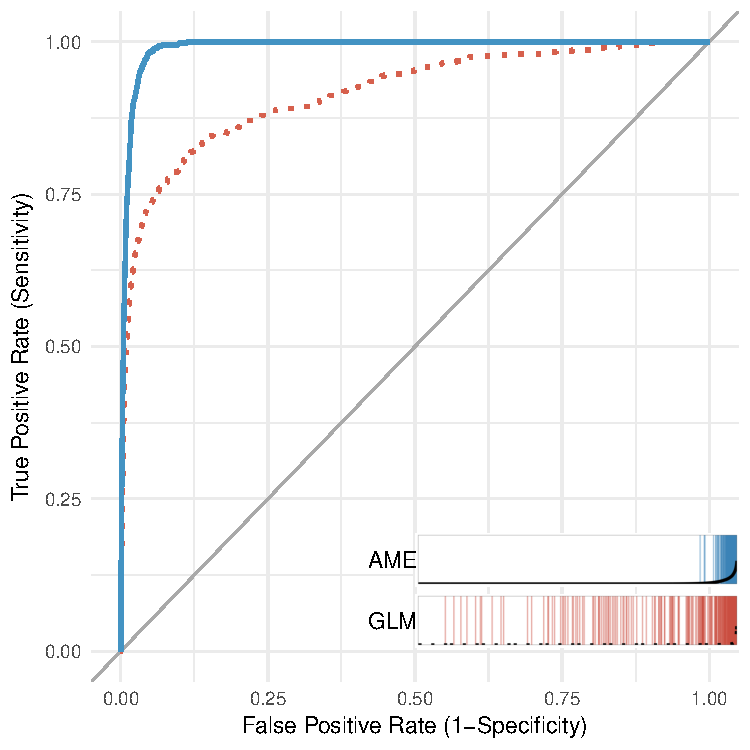
\includegraphics[width=.45\textwidth]{mcdonald_roc_outSample.pdf}}
% 	\subfigure[Precision and Recall]{\label{fig:reitpr}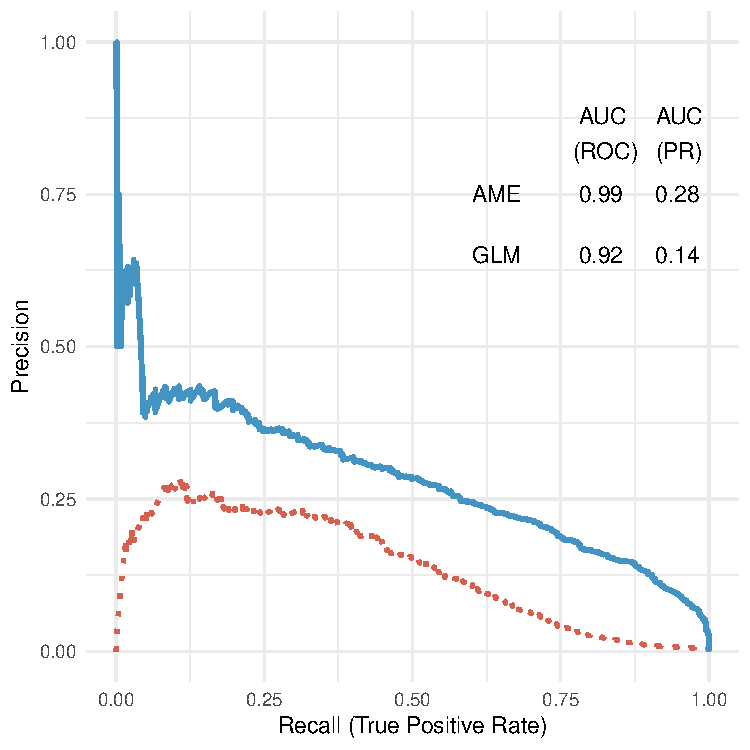
\includegraphics[width=.45\textwidth]{mcdonald_pr_outSample.pdf}}
% 	\caption{Assessments of out-of-sample predictive performance for McDonald (2004) using ROC curves and PR curves.}
% \end{figure}
\FloatBarrier

\clearpage
\subsubsection*{Weeks (2012)}

%Coefficient plot and performance comparison.

% latex table generated in R 3.4.1 by xtable 1.8-2 package
% Sat Oct 21 23:26:08 2017
\begin{table}[ht]
\centering
\begingroup\scriptsize
\begin{tabular}{lccc}
 Variable & GLM (Logit) & GLM (Probit) & AME \\ 
  \hline
\hline
(Intercept) & $-3.784^{\ast\ast}$ & $-1.797^{\ast\ast}$ & $-2.409^{\ast\ast}$ \\ 
   & (0.423) & (0.159) & (0.132) \\ 
  Machine & $-0.459^{\ast\ast}$ & $-0.162^{\ast\ast}$ & -0.006 \\ 
   & (0.174) & (0.062) & (0.04) \\ 
  Junta & $0.515^{\ast\ast}$ & $0.194^{\ast\ast}$ & 0.034 \\ 
   & (0.169) & (0.062) & (0.046) \\ 
  Boss & $0.649^{\ast\ast}$ & $0.281^{\ast\ast}$ & -0.044 \\ 
   & (0.153) & (0.05) & (0.044) \\ 
  Strongman & $0.832^{\ast\ast}$ & $0.295^{\ast\ast}$ & 0.032 \\ 
   & (0.132) & (0.048) & (0.044) \\ 
  Other Type & 0.147 & 0.051 & -0.01 \\ 
   & (0.132) & (0.046) & (0.034) \\ 
  New/Unstable Regime & $-0.312^{\ast\ast}$ & $-0.123^{\ast\ast}$ & -0.043 \\ 
   & (0.092) & (0.033) & (0.031) \\ 
  Democracy Target & 0.185 & 0.052 & 0.024 \\ 
   & (0.115) & (0.04) & (0.026) \\ 
  Military Capabilities Initiator & $5.234^{\ast\ast}$ & $2.136^{\ast\ast}$ & 0.071 \\ 
   & (1.69) & (0.554) & (0.412) \\ 
  Military Capabilities Target  & $6.34^{\ast\ast}$ & $2.865^{\ast\ast}$ & $-0.969^{\ast\ast}$ \\ 
   & (1.675) & (0.573) & (0.48) \\ 
  Low Trade Dependence  & $-24.794^{\ast}$ & -8.197 & -4.733 \\ 
   & (12.866) & (5.582) & (3.017) \\ 
  Both Major Powers & $1.136^{\ast\ast}$ & $0.687^{\ast\ast}$ & $1.122^{\ast\ast}$ \\ 
   & (0.547) & (0.183) & (0.241) \\ 
  Minor/Major & $0.772^{\ast\ast}$ & $0.292^{\ast\ast}$ & $0.496^{\ast\ast}$ \\ 
   & (0.239) & (0.086) & (0.118) \\ 
  Major/Minor & $0.711^{\ast\ast}$ & $0.332^{\ast\ast}$ & $0.778^{\ast\ast}$ \\ 
   & (0.225) & (0.075) & (0.16) \\ 
  Contiguous & $2.172^{\ast\ast}$ & $0.738^{\ast\ast}$ & $0.705^{\ast\ast}$ \\ 
   & (0.32) & (0.125) & (0.06) \\ 
  Log Dist. Between Capitals & $-0.209^{\ast\ast}$ & $-0.095^{\ast\ast}$ & $-0.129^{\ast\ast}$ \\ 
   & (0.038) & (0.015) & (0.01) \\ 
  Alliance Similarity Dyad  & $-0.999^{\ast\ast}$ & $-0.386^{\ast\ast}$ & -0.073 \\ 
   & (0.144) & (0.05) & (0.065) \\ 
  Alliance Similarity With System Leader Initiator & 0.11 & 0.011 & 0.068 \\ 
   & (0.24) & (0.082) & (0.057) \\ 
  Alliance Similarity Leader Target & 0.203 & 0.032 & 0.08 \\ 
   & (0.244) & (0.081) & (0.056) \\ 
  Time Since Last Conflict & $-0.229^{\ast\ast}$ & $-0.089^{\ast\ast}$ & $-0.067^{\ast\ast}$ \\ 
   & (0.018) & (0.007) & (0.007) \\ 
  Spline1 & $-0.001^{\ast\ast}$ & $0.000^{\ast\ast}$ & $0.000^{\ast\ast}$ \\ 
   & (0.000) & (0.000) & (0.000) \\ 
  Spline2 & $0.000^{\ast\ast}$ & $0.000^{\ast\ast}$ & $0.000^{\ast\ast}$ \\ 
   & (0.000) & (0.000) & (0.000) \\ 
  Spline3 & 0.000 & 0.000 & 0.000 \\ 
   & (0.000) & (0.000) & (0.000) \\ 
   \hline
\hline
\end{tabular}
\endgroup
\caption{Parameter comparison for Weeks (2012). Standard errors in parentheses. $^{**}$ and $^{*}$ indicate significance at $p<0.05$ and $p<0.10$, respectively.} 
\label{tab:weeks_coef}
\end{table}

\FloatBarrier

% already show roc-pr in main text
% \begin{figure}
% 	\centering   
% 	\subfigure[AUC]{\label{fig:weeksroc}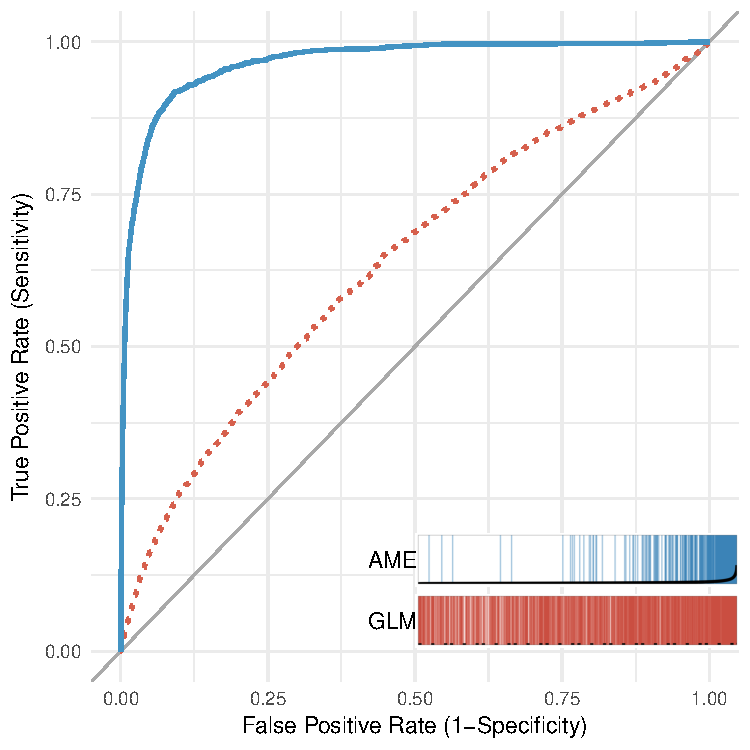
\includegraphics[width=.45\textwidth]{weeks_roc_outSample.pdf}}
% 	\subfigure[Precision and Recall]{\label{fig:weekspr}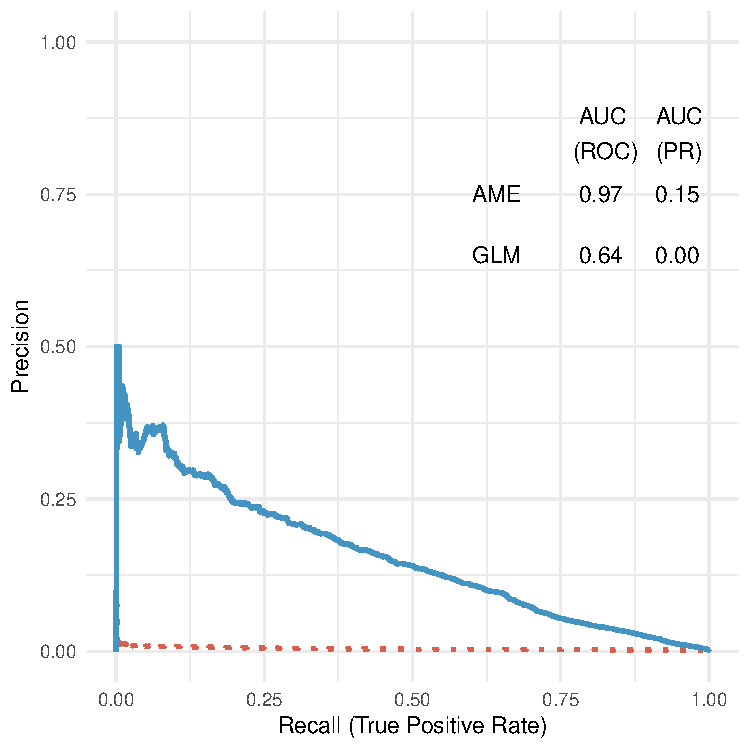
\includegraphics[width=.45\textwidth]{weeks_pr_outSample.pdf}}
% 	\caption{Assessments of out-of-sample predictive performance for Weeks (2012) using ROC curves and PR curves.}
% \end{figure}
% \FloatBarrier